

\section{Theoretical Framework}

\begin{figure}[!htbp]
	\centering
		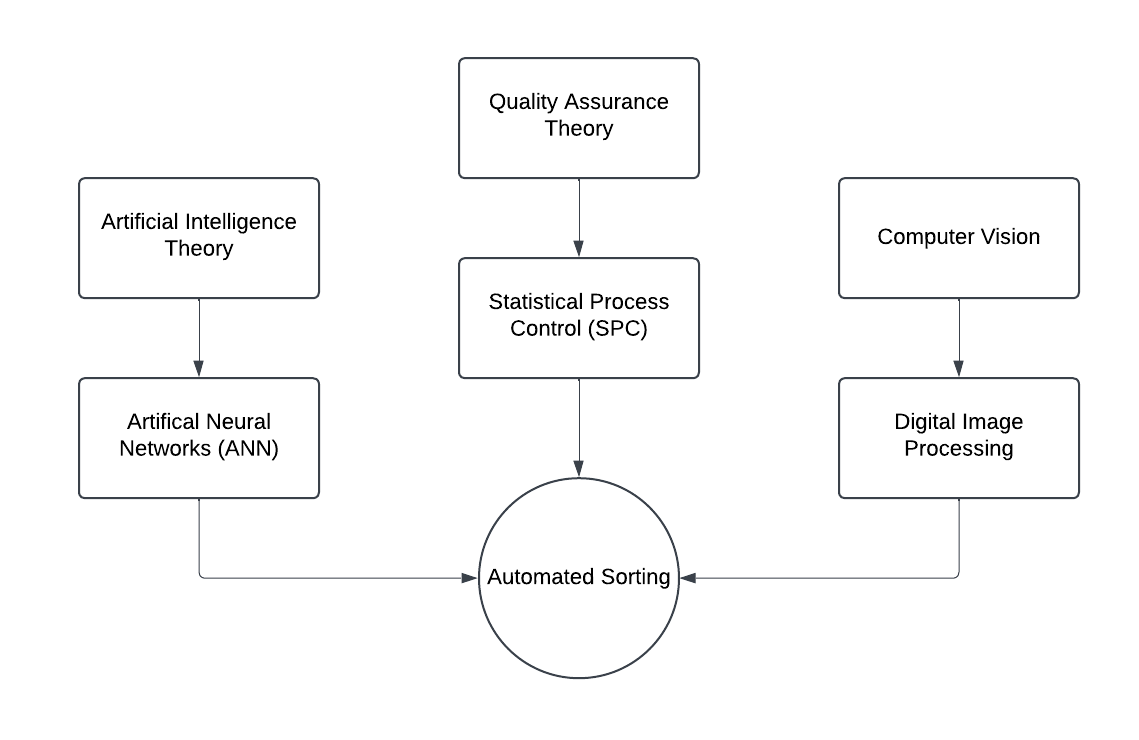
\includegraphics[width=0.8\textwidth]{figure/theoretical_framework.png}
	\caption{Theoretical Framework}
	\label{fig:theoretical_framework}
\end{figure}

The theoretical framework discusses the multiple concepts that are involved in this study. These key concepts are crucial to ensuring the success of the thesis. There are three main concepts that are key to this study, the Artificial Intelligence Theory, the Quality Assurance Theory and lastly, Computer Vision.

\section{Conceptual Framework}

\begin{figure}[!htbp]
	\centering
		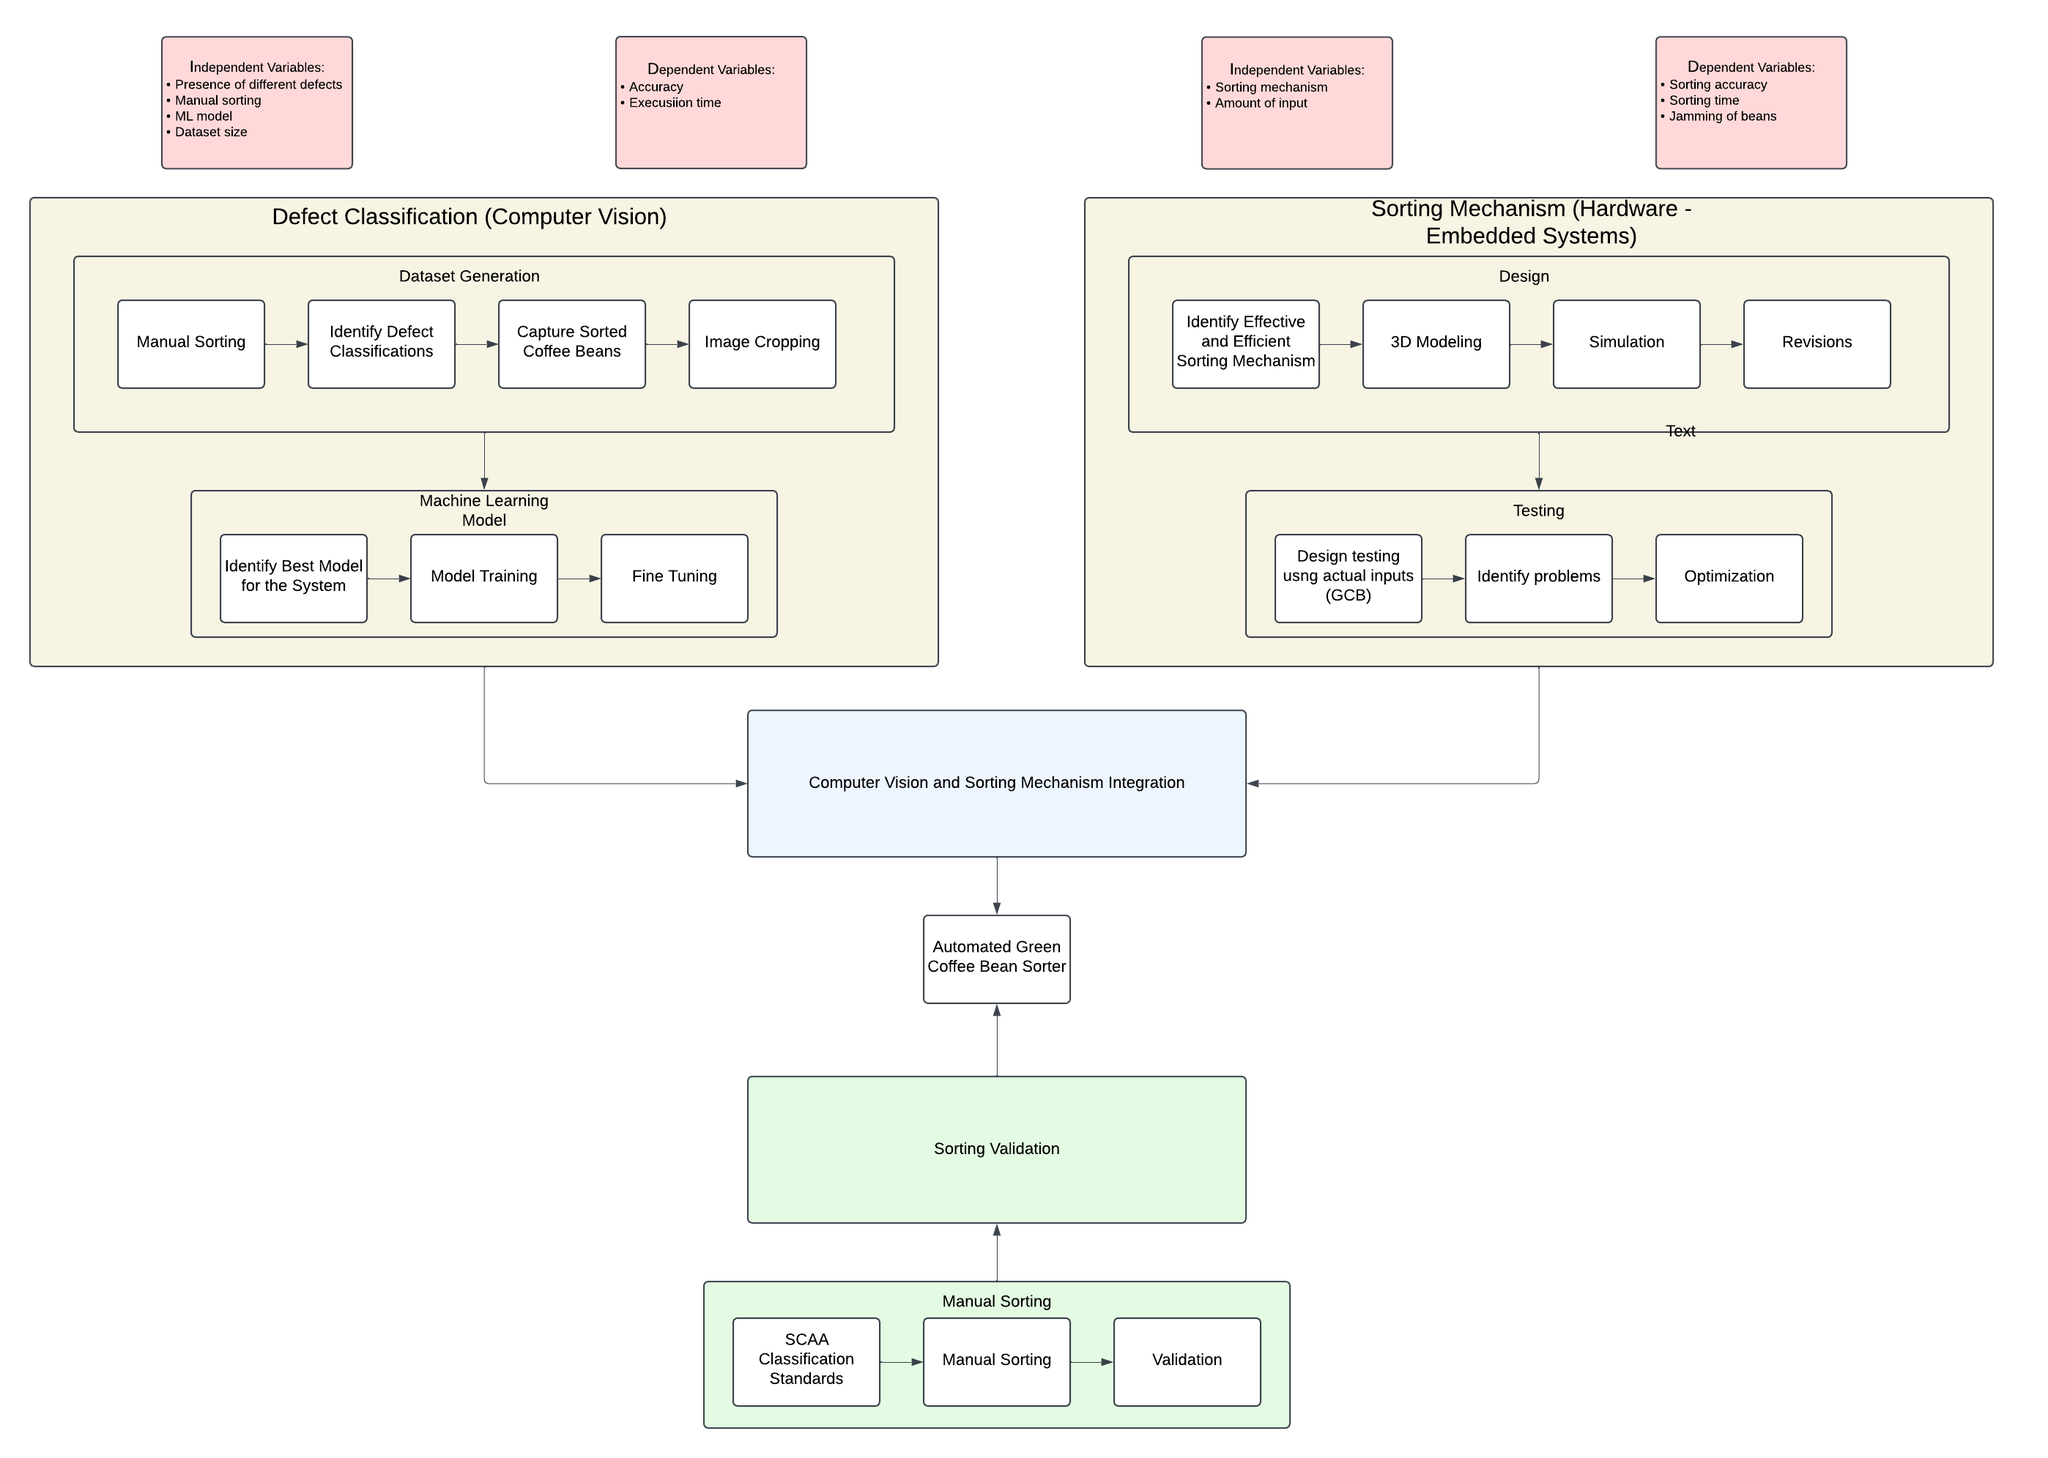
\includegraphics[width=0.8\textwidth]{figure/conceptual_framework.png}
	\caption{Conceptual Framework}
	\label{fig:conceptual_framework}
\end{figure}

The conceptual framework shows the implementation of two systems which consists of machine vision and embedded systems. The framework describes the thought process of both systems with the end goal of integrating both systems. The machine vision handles the defect classification of the system, whereas the embedded system handles the sorting of the beans. By integrating both systems together, creates an automated green coffee bean sorter. The data validation is done by sorting through the tested coffee beans by the system following the standards of the SCAA.

\section{Summary}